% T4 family (c): a MATRIX+FIT framework MAP — the shape for a dense, multi-stage
% method where you want an aligned overview ("the paper's structure on one page").
% Distilled in framework-figures.md from xinychen/awesome-latex-drawing (Example 25:
% \matrix positions components, \fit groups them into labelled bands).
%
% Build:  pdflatex matrix_layout_hero.tex   ->  matrix_layout_hero.pdf
% Paper:  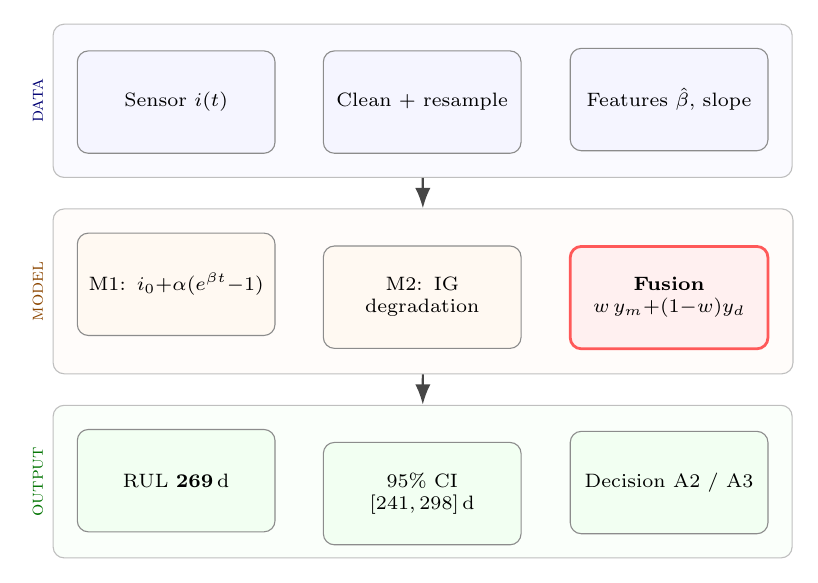
\includegraphics[width=.75\linewidth]{matrix_layout_hero.pdf}
%
% Technique: \matrix of nodes lays the grid; \fit (on the background layer) wraps
% each row into a labelled band; the hero cell is the heaviest. To stay on the
% right side of the §0b axis-1 rule (a layout of empty boxes IS the generic
% flowchart we warn against), every cell carries a REAL artifact — a formula, a
% number — not a bare label, so the map doubles as the paper's result ledger.
\documentclass[border=3mm]{standalone}
\usepackage{tikz}
\usepackage{amsmath, amssymb}
\usetikzlibrary{matrix, fit, positioning, arrows.meta, backgrounds, calc}
\begin{document}
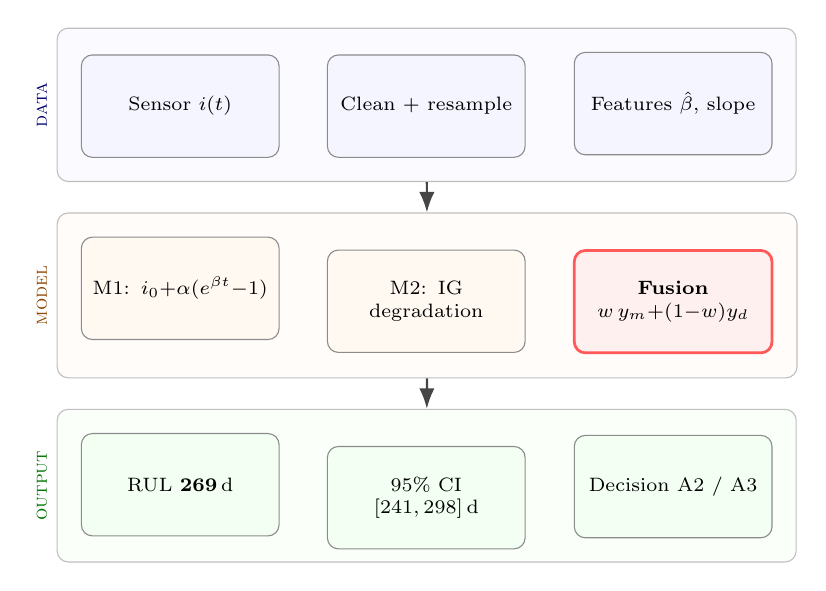
\begin{tikzpicture}[
  dat/.style ={fill=blue!4},
  mdl/.style ={fill=orange!5},
  res/.style ={fill=green!5},
  hero/.style={draw=red!65, line width=1pt, fill=red!6},
  band/.style={rounded corners, inner sep=3mm, draw=black!25},
  arr/.style ={-{Latex[length=2.6mm]}, thick, gray!55!black},
]
  % (in `matrix of nodes`, \\ ends a ROW — never put \\ inside a cell; let
  %  text width wrap the content instead)
  \matrix (m) [matrix of nodes,
    nodes={draw=black!45, rounded corners, align=center, font=\scriptsize,
           minimum height=13mm, text width=23mm, inner sep=3pt},
    row sep=10mm, column sep=6mm]{
    |[dat]|  Sensor $i(t)$ & |[dat]|  Clean + resample & |[dat]|  Features $\hat\beta$, slope \\
    |[mdl]|  M1: $i_0{+}\alpha(e^{\beta t}{-}1)$ & |[mdl]|  M2: IG degradation & |[hero]| \textbf{Fusion} $w\,y_m{+}(1{-}w)y_d$ \\
    |[res]|  RUL \textbf{269}\,d & |[res]|  95\% CI $[241,298]$\,d & |[res]|  Decision A2 / A3 \\
  };

  % --- fit each row into a labelled band (technique: \fit on background layer) -
  \begin{scope}[on background layer]
    \node[band, fill=blue!2,   fit=(m-1-1)(m-1-3),
          label={[font=\scriptsize, text=blue!45!black]left:\rotatebox{90}{\textsc{data}}}]  (bD) {};
    \node[band, fill=orange!2, fit=(m-2-1)(m-2-3),
          label={[font=\scriptsize, text=orange!55!black]left:\rotatebox{90}{\textsc{model}}}] (bM) {};
    \node[band, fill=green!2,  fit=(m-3-1)(m-3-3),
          label={[font=\scriptsize, text=green!45!black]left:\rotatebox{90}{\textsc{output}}}] (bO) {};
  \end{scope}

  % --- flow between bands ----------------------------------------------------
  \draw[arr] (bD) -- (bM);
  \draw[arr] (bM) -- (bO);
\end{tikzpicture}
\end{document}
